\documentclass[11pt]{report}
\usepackage{amsmath, amsthm, amssymb, amsfonts}
\usepackage[a4paper,margin=1in,footskip=0.25in]{geometry}
\usepackage{float}
\usepackage{graphicx}
\usepackage{comment}
\usepackage{enumitem}
\setlength\parindent{0pt}
\begin{document}



\section*{Call Center Data Modeling}
Complete the call center data modeling assignment we start in the Pre­class work and Activity 2
breakouts of Session 2.2. You may re­use and build on all code or any other work from the class
session.\\ 

In class we completed the Bayesian data modeling problem for 1 hour of the day. In this
assignment you need to do the same analysis for all 24 hours of the day.

\begin{enumerate}
	\item Compute a 95\% posterior confidence interval over the number of calls per minute (the call rate $\lambda$ ) for each hour of the day — so you will have 24 confidence intervals. Also compute the posterior mean of $\lambda$ for each hour of the day.
	\begin{verbatim}
		alpha_prior, beta_prior = 1, 0.25

errors = []

for x in waiting_times_per_hour:
    alpha_posterior, beta_posterior = alpha_prior + len(x), beta_prior + sum(x)
    posterior = stats.gamma(a=alpha_posterior, scale=1/beta_posterior)
    errors.append((posterior.ppf(0.975) - posterior.ppf(0.025))/2) \end{verbatim}
    \item Present your results graphically using Matplotlib. Make a plot that looks like the one below. Each dot is at the posterior mean and each line shows a 95\% confidence e interval for a λ. You can use the \texttt{errorbar()} function in the plotting library to do this. 
    \begin{verbatim}
plt.errorbar(np.arange(24), 
             np.array([len(w) for w in waiting_times_per_hour])/60, 
             yerr=errors, fmt='o')
plt.show()
	\end{verbatim}
\begin{figure}[H]
  \centering
    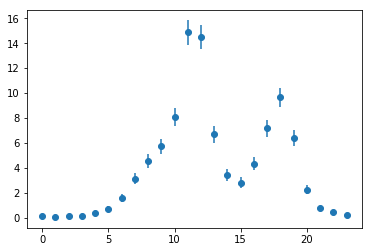
\includegraphics[width=0.5\textwidth]{confint.png}
    \end{figure}
    \item Write a paragraph (100 - 200 words) to accompany your plot and present your findings to the client. Carefully summarize how many calls you expect during different parts of the day, and how much uncertainty there is in your estimates. Remember that the client is not an expert in statistics, so make it easy for them to understand. You may also make additional plots to help communicate your results. \newpage We see that the number of calls per minute follow a very specific pattern - there are relatively few calls per minute during the early hours of the morning until around 7am, where the calls per minute jump rapidly from 5 per minute to around 15 at 11am. The most calls occur in a one-hour period occur between 11am and 12pm, before dipping to a low of around 2.5 calls per minute at 3 in the afternoon, and rising again to a small peak of 10 calls per minute at 6pm. After 7pm, the calls once again drop to a meagre rate of 1-2 per minute. As the number of calls are increased, our margin of error for the call rates also necessarily widen. Because of the small number of calls during the 1am-2am period, for example, very few calls are made, so an estimate of 0 per minute will not significantly deviate from the true figure. At 11am, however, the larger number of calls means the true rate could vary from 13-16 calls per minute, depending on the day.
\end{enumerate}
\section*{Stretch Goals}
\begin{enumerate}
	\item Reparameterize the normal likelihood function in terms of the precision parameter, $\tau = 1/\sigma^2$. \\ $$ f(x | \mu, \sigma^2) = \frac{1}{\sqrt{2\pi\sigma^2}} e^{-\frac{(x - \mu)^2}{2 \sigma^2}} \implies f(x \mid  \mu,\tau ) =  \sqrt{\frac{\tau}{2\pi }}e^{- \tau \frac{(x - \mu)^2}{2}} $$
	\item Prove that if you substitute into the normal­-inverse-­gamma pdf $ \sigma = 1 / \sqrt{\tau}$ , you get the normal­ - gamma pdf, which is the conjugate prior for the normal likelihood with unknown mean $\mu$ and precision $\tau$.  \begin{align*} 
 	f(x,\sigma^2\mid\mu,\lambda,\alpha,\beta) &=  \frac {\sqrt{\lambda}} {\sigma\sqrt{2\pi} } \, \frac{\beta^\alpha}{\Gamma(\alpha)} \, \left( \frac{1}{\sigma^2} \right)^{\alpha + 1}   \exp \left( -\frac { 2\beta + \lambda(x - \mu)^2} {2\sigma^2} \bigg) \\
 \implies f(x,\tau \mid\mu,\lambda,\alpha,\beta) &= \frac{\beta^\alpha \sqrt{\lambda}}{\Gamma(\alpha)\sqrt{2\pi}}  \, \tau^{\alpha-\frac{1}{2}}\,e^{-\beta\tau}\,e^{ -\frac{ \lambda \tau (x- \mu)^2}{2}} \end{align*} The main difficulty in this question is in finding the correct power of $\tau$. From the $\sigma$ in the denominator, we have $\tau^{1/2}.$ From the middle term, we have $\tau^{\alpha + 1}$. From $\big|\frac{d\sigma}{d\tau} \big|$, we have $\big|-\tau^{-2}\big| = \tau^{-2}$. The resultant power is $1/2 + \alpha + 1 - 2 = \alpha - 1/2$.
	\item As part of this transformation you will have to multiply by $\big|\frac{d\sigma}{d\tau} \big|$. Explain why this is needed in your own words and so that a student who has not yet encountered this concept can understand it. \\ \\ When integrating by substitution of a new variable, we use the formula: $$ P(a \leq X < b)=  \int_{a}^{b} f(x) \ dx = \int_{f(a)}^{f(b)}f(x(y)) \ \frac{dx}{dy} \ d(y) = P\big(y(a) \leq Y < y(b)\big)$$ The PDF of X is found in its integrand, $f(x)$. Likewise, the integrand of Y is: $$ P(y(a) \leq Y < y(b)) = \int_{y(a)}^{y(b)}g(y) \  dy , \quad \textrm{where} \  g(y) = f(x(y)) \ \frac{dx}{dy} \ }$$ However, the derived PDF is often used with the derivated inside a modulus: $$g(y) = f(x(y)) \bigg|\frac{dx}{dy} \bigg| $$ This is because there are constraints on the PDF $f(x)$: \begin{itemize}
 \item $f(x)$ must be single valued for all $x$.
 \item $f(x) \geq 0$ for all $x$.
 \item $\int_{- \infty}^{\infty} f(x) \ dx = 1	$
 \end{itemize} As a result, $y(x)$ and $x(y)$ must be defined and single-valued, and $\frac{dx}{dy} \geq 0$ or $\frac{dx}{dy} \leq 0$. In other words, a practically useful transformation $y(x)$ must be either monotonically increasing or decreasing over the range of $x$, otherwise its inverse would be multi-valued.


\end{enumerate}


\end{document}
